\def \kaflanr {20}
\lecture[\kaflanr]{\kaflanr. Fletir}{lecture-text}
\date{11.~mars 2015}
\newcounter{mycount}
\refstepcounter{mycount}

\begin{document}

\begin{frame}
	\maketitle
\end{frame}




\begin{frame}{Fletir} 

\begin {block}{Óformleg skilgreining  \rtask{}}
Flötur $\cal S$ í $\R^3$ er
,,tvívítt\lq\lq\ hlutmengi í $\R^3$.   
\end{block}

\end{frame}


\begin{frame}{Fletir} 

\begin {block}{Lýsing  \rtask{}}
Flötum er aðallega lýst með formúlum á þrjá vegu:

\begin{enumerate}
 \item Gefið er fall $f(x,y,z)$.  Fletinum $\cal S$ er lýst með jöfnu 
$f(x,y,z)=C$ (þ.e.a.s.~$\cal S$ er jafnhæðarflötur fallsins $f$).  Þá
er
$${\cal S}=\{(x,y,z)\mid f(x,y,z)=C\}.$$

\item Gefið er fall skilgreint á ferilsamanhangandi 
svæði $D$ í $\R^2$.  Fletinum $\cal S$
er lýst sem grafi fallsins $f$.  Þá er
$${\cal S}=\{(x,y,z)\mid (x,y)\in D\mbox{ og } z=f(x,y)\}.$$

\item Með stikafleti (sjá næstu glæru). 
\end{enumerate}

\end{block}

\end{frame}



\begin{frame}{Stikafletir} 

\begin {block}{Skilgreining  \rtask{}}

Látum $D$ vera ferilsamanhangandi hlutmengi í $\R^2$.  Samfelld vörpun
$\rv:D\rightarrow \R^3; \rv (u,v)=\big(x(u,v), y(u,v), z(u,v)\big)$  
þannig að  
$${\cal S}=\{\rv(u,v)\mid (u,v)\in D\}$$
er flötur kallast {\em stikaflötur}.  Segjum að $\rv$ sé {\em stikun á
  fletinum} $\cal S$. 
Viljum að $\rv$ sé eintæk vörpun, nema hugsanlega á jaðri $D$.
Ritum einnig 
$$\frac{\partial \rv}{\partial u}=
\bigg(\frac{\partial x}{\partial u}, \frac{\partial y}{\partial u},
\frac{\partial z}{\partial u}\bigg)\quad\mbox{ og }\quad
\frac{\partial \rv}{\partial v}=
\bigg(\frac{\partial x}{\partial v}, \frac{\partial y}{\partial v},
\frac{\partial z}{\partial v}\bigg).$$
\end{block}

\end{frame}


\begin{frame}{Snertiplön} 

\begin {block}{Setning  \rtask{snertifletir}}
\begin {enumerate}
 \item  Látum $\cal S$ vera flöt sem er gefinn sem jafnhæðarflötur 
     $f(x,y,z)=C$.   Ef $(a, b, c)$ er punktur á fletinum og
     fallið $f$ er diffranlegt í punktinum $(a, b,c)$ þá er vigurinn
     $\nv=\nabla f(a, b, c)$ hornréttur á flötinn í punktinum $(a,
    b, c)$ og ef $\nabla f(a, b, c)\neq \ov$ þá hefur
flöturinn snertiplan í punktinum.  Jafna
     snertiplansins er
$$f_1(a, b, c)x+f_2(a, b, c)y+f_3(a, b, c)z=D$$ 
þar sem 

$$D= f_1(a, b, c)a+f_2(a, b, c)b
+f_3(a, b, c)c.$$

\end {enumerate}

\end{block}

\end{frame}

\begin{frame}{Snertiplön}
 \begin {block}{Setning \kaflanr.\ref{snertifletir}, frh.}
   \begin {enumerate}
    \item [2.] 
   Látum $\cal S$ vera flöt sem er gefinn sem graf falls 
     $z=f(x,y)$.   Ef $(a, b, f(a,b))$ er punktur á fletinum og
     fallið $f$ er diffranlegt í punktinum $(a, b)$ þá er vigurinn
     
     $$\nv =\big(0 ,1 ,f_2(a, b)\big)\times\big(1 ,0 ,f_1(a, b)\big)
=\big(f_1(a, b), f_2(a, b), -1\big)$$ 

hornréttur á flötinn í punktinum $(a,
     b, f(a,b))$ og flöturinn hefur snertiplan í punktinum.  Jafna
     snertiplansins er
$$z=f(a, b)+f_1(a, b)(x-a)+f_2(a, b)(y-b).$$
   \end {enumerate}

 \end {block}

\end{frame}

\begin {frame}{Snertiplön}
 \begin{figure}[!h]
        \centering
        \begin{minipage}{.5\textwidth}
            \centering
            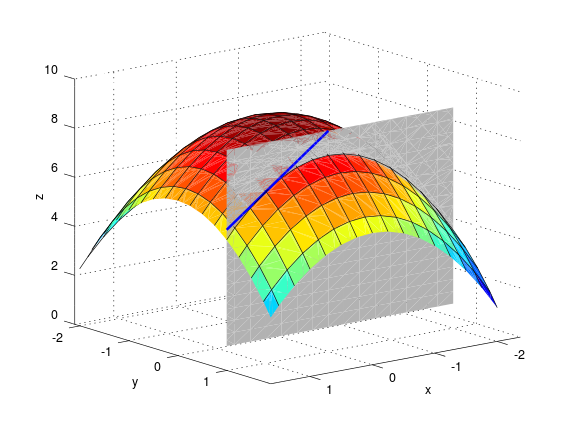
\includegraphics[width=1\linewidth]{xpart.png}
            \caption*{Snertivigur við skurðferil sléttunnar \\ $y=b$ og yfirborðsins $z = f(x,y)$ \\ í punktinum $(a,b,f(a,b))$ er \\ $\mathbf{T}_1 = (1,0,f_1(a,b))$.}
        \end{minipage}%
        \begin{minipage}{.5\textwidth}
            \centering
            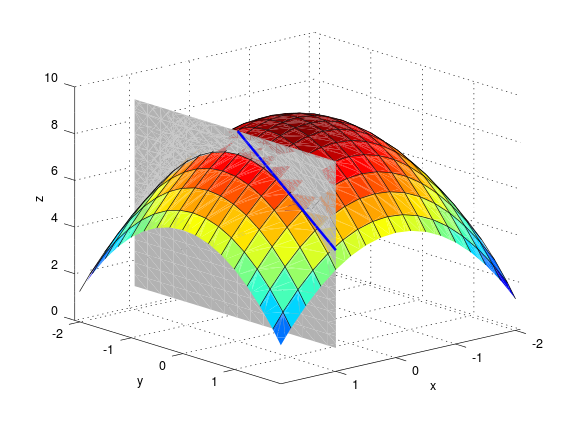
\includegraphics[width=1\linewidth]{ypart.png}
            \caption*{Snertivigur við skurðferil sléttunnar \\ $x=a$ og yfirborðsins $z = f(x,y)$ \\ í punktinum $(a,b,f(a,b))$ er \\ $\mathbf{T}_2 = (0,1,f_2(a,b))$.}
        \end{minipage}
    \end{figure}
 
\end {frame}


\begin{frame}{Snertiplön}
 \begin {block}{Setning \kaflanr.\ref{snertifletir}, frh.}
     \begin {enumerate}
    \item [3.] 
  Látum $\rv: D\subseteq \R^2\rightarrow \R^3$ vera stikaflöt.  
Ef $(x_0, y_0, z_0)=\rv(u_0, v_0)$ er punktur á fletinum sem 
$\rv(u,v)=\big(x(u,v), y(u,v), z(u,v)\big)$ stikar og
föllin $x(u,v), y(u,v), z(u,v)$ eru diffranleg í punktinum $(x_0,
y_0)$ þá er vigurinn
     $$\nv =\frac{\partial \rv}{\partial u}\times 
\frac{\partial \rv}{\partial v}$$
reiknaður með $u=u_0$ og $v=v_0$ þvervigur á flötinn í punktinum 
$(x_0, y_0, z_0)$.
\end {enumerate}
 \end {block}

\end{frame}

\begin{frame}{Snertiplön} 

\begin {block}{Skilgreining  \rtask{}}
Ef vigrarnir $\frac{\partial \rv}{\partial
  u}(u,v)$ og    $\frac{\partial \rv}{\partial v}(u,v)$ eru óháðir
fyrir alla punkta $(u,v)\in D$ þá er sagt að stikunin sé {\em
  regluleg}. 

 
\end{block}

\end{frame}



\begin{frame}{Snertiplön} 

\begin {block}{Athugasemd \rtask{}}
Ef vigrarnir  
$\frac{\partial \rv}{\partial u}(u_0,v_0)$ og    $\frac{\partial
  \rv}{\partial v}(u_0,v_0)$ eru óháðir þá spanna þeir snertiplan við
flötinn í punktinum $\rv(u_0,v_0)$. Snertiplanið hefur stikun 

$$\Pi(u,v) = \rv(u_0,v_0)+u\frac{\partial \rv}{\partial u}(u_0,v_0)
+v\frac{\partial \rv}{\partial v}(u_0,v_0).$$

\end{block}

\end{frame}


\begin{frame}{Flatarheildi} 

\begin {block}{Verkefni  \rtask{}}
\begin {enumerate}
 \item Flatarmál flata -- sambærilegt við bogalengd ferla.  
\item Heildi falls yfir flöt með tilliti til flatarmáls -- sambærilegt við heildi falls eftir ferli með tilliti til bogalengdar.
\item Heildi vigursviðs yfir flöt -- svipar til heildis vigursviðs eftir ferli. 
 \end {enumerate}



\end{block}

\end{frame}



\begin{frame}{Flatarmál flata} 

\begin {block}{Skilgreining  \rtask{}}
  Látum $\rv:D\rightarrow \R^2$ vera
reglulegan stikaflöt sem stikar flöt $\cal S$.  Flatarmál $\cal S$ er  
$$ A=\tvint_D\,dS=\tvint_D \big|{\textstyle\frac{\partial \rv}{\partial u}
\times\frac{\partial \rv}{\partial v}}\big|\,dudv.$$
\end{block}

\end{frame}


\begin{frame}{Flatarmál flata} 

\begin {block}{Formúla  \rtask{}}
Látum $f(x,y)$ vera diffranlegt fall skilgreint á
mengi $D$ í $\R^2$.  Flatarmál grafsins $z=f(x,y)$ er gefið með
formúlunni 
$$A=\tvint_D dS=\tvint_D {\textstyle\sqrt{1+
\big(\frac{\partial f}{\partial x}\big)^2+
\big(\frac{\partial f}{\partial y}\big)^2}}\,\,dx\,dy.$$
   
\end{block}

\end{frame}

\end{document}